\documentclass[12pt]{article}
\newif\ifanswer\answertrue%\answerfalse% comment out to show/hide answers
\usepackage{../preamble3}% preamble always after \newif\ifanswer
%\pagenumbering{gobble}
\title{Art Of Problem Solving - AMC 10 \\ July 31, 2021}
\author{Patrick \& James Toche}
\date{Revised:~\today}

\begin{document}
\maketitle
\begin{minipage}{\textwidth}
\begin{abstract}\setlength{\parindent}{0pt}%
Notes on the AMC-10 Course by Art Of Problem Solving (AOPS).
Copyright restrictions may apply. Written for personal use. 
Please report typos and errors over at \url{https://github.com/ptoche/Math/tree/master/aops}. 
\end{abstract}
\end{minipage}

\thispagestyle{empty}
\clearpage


%%%%%%%%%%%%%%%%%%%%%%%%%%%%%%%%%%%%%%%%%%%%%%%%%%%%%%%%%%%%%%%%%%%%%%%%
\subsection*{1.}

\nopagebreak

A solid cube has side length 3 inches. A 2-inch by 2-inch square hole is cut into the center of each face. The edges of each cut are parallel to the edges of the cube, and each hole goes all the way through the cube. What is the volume, in cubic inches, of the remaining solid?

\fbox{(A) $7$ \quad (B) $8$ \quad (C) $10$ \quad (D) $12$ \quad (E) $15$}

\begin{answer}
Imagine making the cuts one at a time. The first cut removes a box $2\times 2\times 3$. The second cut removes two boxes, each of dimensions $2\times 2\times 0.5$, and the third cut does the same as the second cut, on the last two faces. Hence the total volume of all cuts is $12 + 4 + 4 = 20$.

Therefore the volume of the rest of the cube is
\begin{align*}
3^3 - 20 = 27 - 20 = 7
\end{align*}
\begin{empheq}[box={\mathbox[colback=white]}]{equation*}
    7
\end{empheq} 
\end{answer}
%%%%%%%%%%%%%%%%%%%%%%%%%%%%%%%%%%%%%%%%%%%%%%%%%%%%%%%%%%%%%%%%%%%%%%%%

\iftoggle{showAnswers}{\newpage}

%%%%%%%%%%%%%%%%%%%%%%%%%%%%%%%%%%%%%%%%%%%%%%%%%%%%%%%%%%%%%%%%%%%%%%%%
\subsection*{2.}

\nopagebreak

Consider the 12-sided polygon $ABCDEFGHIJKL$, as shown. Each of its sides has length 4, and each two consecutive sides form a right angle. Suppose that $AG$ and $CH$ meet at $M$. What is the area of quadrilateral $ABCM$?

\bigskip
\begin{center}
  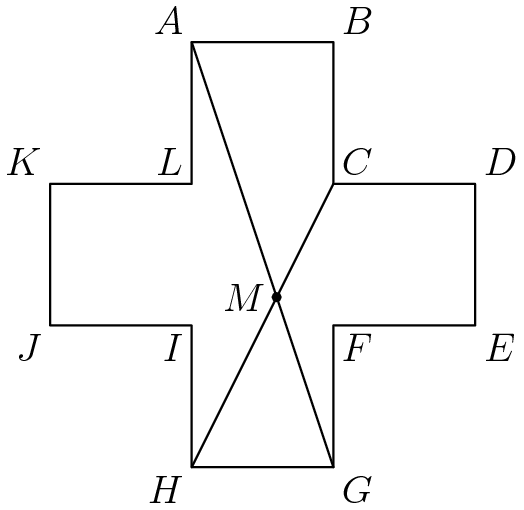
\includegraphics[height=5cm,page=1]{2021-07-31-figure-02}
\end{center}
\bigskip

\fbox{(A) $\dfrac{44}{3}$ \quad (B) $16$ \quad (C) $\dfrac{88}{5}$ \quad (D) $20$ \quad (E) $\dfrac{62}{3}$}

\begin{answer}
We can obtain the solution by calculating the area of rectangle $ABGH$ minus the combined area of triangles $\triangle AHG$ and $\triangle CGM$.

We know that triangles $\triangle AMH$ and $\triangle GMC$ are similar because $\overline{AH} \parallel \overline{CG}$. Also, since $\frac{AH}{CG} = \frac{3}{2}$, the ratio of the distance from $M$ to $\overline{AH}$ to the distance from $M$ to $\overline{CG}$ is also $\frac{3}{2}$. Solving with the fact that the distance from $\overline{AH}$ to $\overline{CG}$ is 4, we see that the distance from $M$ to $\overline{CG}$ is $\frac{8}{5}$.

The area of $\triangle AHG$ is simply $\frac{1}{2} \cdot 4 \cdot 12 = 24$, the area of $\triangle CGM$ is $\frac{1}{2} \cdot \frac{8}{5} \cdot 8 = \frac{32}{5}$, and the area of rectangle $ABGH$ is $4 \cdot 12 = 48$.

Taking the area of rectangle $ABGH$ and subtracting the combined area of $\triangle AHG$ and $\triangle CGM$ yields
\begin{align*}
48 - \left(24 + \frac{32}{5}\right) 
  = \frac{88}{5}
\end{align*}
\begin{empheq}[box={\mathbox[colback=white]}]{equation*}
    \frac{88}{5}
\end{empheq} 
\end{answer}
%%%%%%%%%%%%%%%%%%%%%%%%%%%%%%%%%%%%%%%%%%%%%%%%%%%%%%%%%%%%%%%%%%%%%%%%

\iftoggle{showAnswers}{\newpage}

%%%%%%%%%%%%%%%%%%%%%%%%%%%%%%%%%%%%%%%%%%%%%%%%%%%%%%%%%%%%%%%%%%%%%%%%
\subsection*{3.}

\nopagebreak

A paint brush is swept along both diagonals of a square to produce the symmetric painted area, as shown. Half the area of the square is painted. What is the ratio of the side length of the square to the brush width?

\bigskip
\begin{center}
  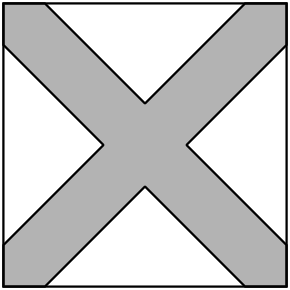
\includegraphics[height=4cm,page=1]{2021-07-31-figure-03}
\end{center}
\bigskip

\fbox{(A) $2\sqrt{2}+1$ \quad (B) $3\sqrt{2}$ \quad (C) $2\sqrt{2}+2$ \quad (D) $3\sqrt{2}+1$ \quad (E) $3\sqrt{2}+2$}

\begin{answer}
Without loss of generality, let the side length of the square be $1$ unit. The area of the painted area is $\frac{1}2$ of the area of the larger square, so the total unpainted area is also $\frac{1}{2}$. Each of the $4$ unpainted triangles has area $\frac{1}8$. It can be observed that these triangles are isosceles right triangles, so let $a$ be the side length of one of the smaller triangles:
\begin{align*}
\frac{a^2}{2} = \frac{1}{8} \rightarrow a = \frac{1}{2}
\end{align*}
The hypotenuse of the triangle is $\frac{\sqrt{2}}{2}$. The corners of the painted area are also isosceles right triangles with side length $\frac{1-\frac{\sqrt{2}}{2}}{2} = \frac{1}{2}-\frac{\sqrt2}4$. Its hypotenuse is equal to the width of the paint, and is $\frac{\sqrt{2}}2-\frac{1}{2}$. The answer we are looking for is thus $\frac{1}{\frac{\sqrt{2}}2-\frac{1}{2}}$. Multiply the numerator and the denominator by $\frac{\sqrt{2}}{2}+\frac{1}{2}$ to simplify, and you get
\begin{align*}
\frac{\frac{\sqrt{2}}{2}+\frac{1}{2}}{\frac{2}{4}-\frac{1}{4}}
= 4\left(\frac{\sqrt{2}}{2}+\frac{1}{2}\right)
= 2\sqrt{2}+2
\end{align*}
\begin{empheq}[box={\mathbox[colback=white]}]{equation*}
    2\sqrt{2}+2
\end{empheq} 
\end{answer}
%%%%%%%%%%%%%%%%%%%%%%%%%%%%%%%%%%%%%%%%%%%%%%%%%%%%%%%%%%%%%%%%%%%%%%%%

\iftoggle{showAnswers}{\newpage}

%%%%%%%%%%%%%%%%%%%%%%%%%%%%%%%%%%%%%%%%%%%%%%%%%%%%%%%%%%%%%%%%%%%%%%%%
\subsection*{4.}

\nopagebreak

A fly trapped inside a cubical box with side length 1 meter decides to relieve its boredom by visiting each corner of the box. It will begin and end in the same corner and visit each of the other corners exactly once. To get from a corner to any other corner, it will either fly or crawl in a straight line. What is the maximum possible length, in meters, of its path?

\fbox{(A) $4+4\sqrt{2}$ \quad (B) $2+4\sqrt{2}+2\sqrt{3}$ \quad (C) $2+3\sqrt{2}+3\sqrt{3}$ \quad (D) $4\sqrt{2}+4\sqrt{3}$ \quad (E) $3\sqrt{2}+5\sqrt{3}$}

\begin{answer}
The path of the fly consists of eight line segments, where each line segment goes from one corner to another corner. The distance of each such line segment is $1$, $\sqrt{2}$, or $\sqrt{3}$.

The only way to obtain a line segment of length $\sqrt{3}$ is to go from one corner of the cube to the opposite corner. Since the fly visits each corner exactly once, it cannot traverse such a line segment twice. Also, the cube has exactly four such diagonals, so the path of the fly can contain at most four segments of length $\sqrt{3}$. Hence, the length of the fly's path can be at most $4\sqrt{3}+4\sqrt{2}$. This length can be achieved by taking the path
\bigskip
\begin{center}
  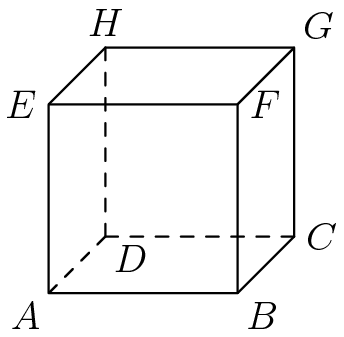
\includegraphics[height=5cm,page=1]{2021-07-31-figure-04}
\end{center}
\begin{align*}
A \rightarrow G \rightarrow B \rightarrow H \rightarrow C \rightarrow E \rightarrow D \rightarrow F \rightarrow A
\end{align*}
\begin{empheq}[box={\mathbox[colback=white]}]{equation*}
    4 \sqrt{3} + 4 \sqrt{2}
\end{empheq} 
\end{answer}
%%%%%%%%%%%%%%%%%%%%%%%%%%%%%%%%%%%%%%%%%%%%%%%%%%%%%%%%%%%%%%%%%%%%%%%%

\iftoggle{showAnswers}{\newpage}
  
%%%%%%%%%%%%%%%%%%%%%%%%%%%%%%%%%%%%%%%%%%%%%%%%%%%%%%%%%%%%%%%%%%%%%%%%
\subsection*{5.}

\nopagebreak

A cube with side length 1 is sliced by a plane that passes through two diagonally opposite vertices $A$ and $C$ and the midpoints $B$ and $D$ of two opposite edges not containing $A$ or $C$, as shown. What is the area of quadrilateral $ABCD$?

\bigskip
\begin{center}
  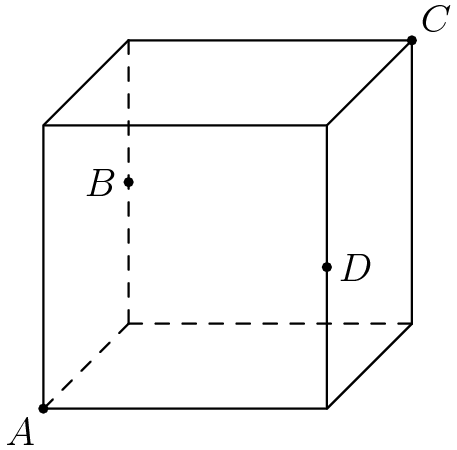
\includegraphics[height=5cm,page=1]{2021-07-31-figure-05}
\end{center}
\bigskip

\fbox{(A) $\dfrac{\sqrt{6}}{2}$ \quad (B) $\dfrac{5}{4}$ \quad (C) $\sqrt{2}$ \quad (D) $\dfrac{3}{2}$ \quad (E) $\sqrt{3}$}

\begin{answer}
\bigskip
\begin{center}
  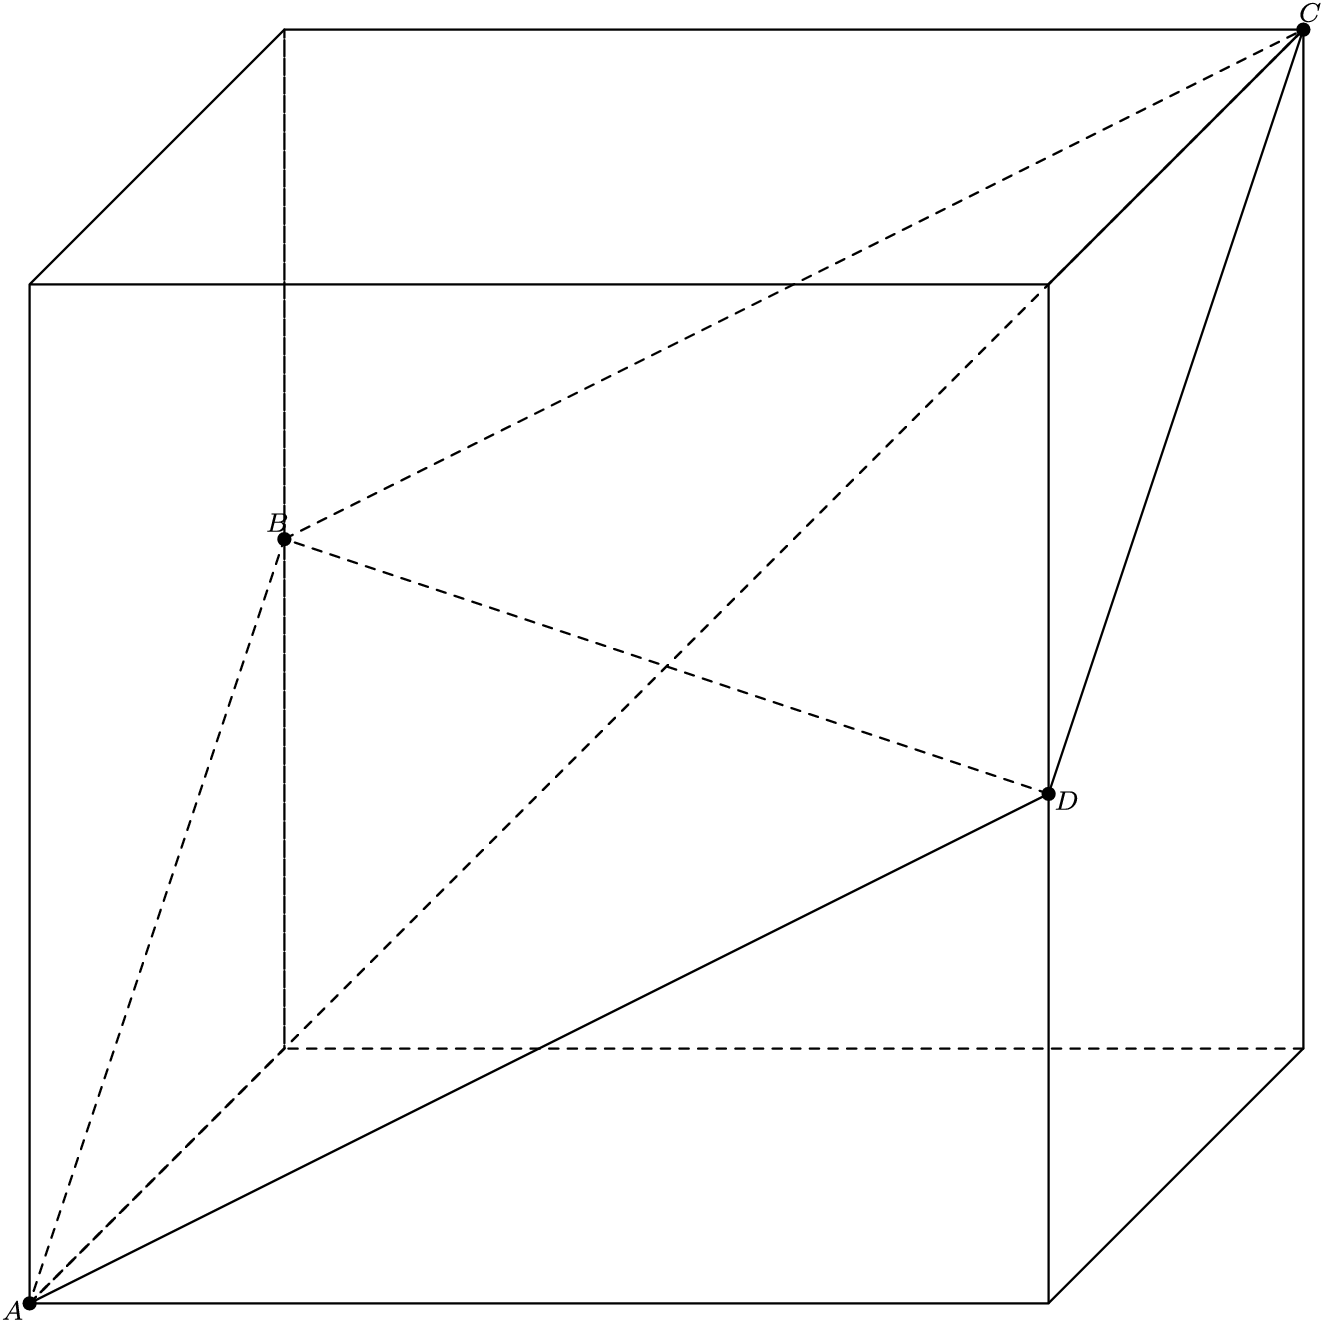
\includegraphics[height=5cm,page=1]{2021-07-31-figure-05b}
\end{center}
\begin{align*}
AB = AD = CB = CD = \sqrt{\left(\frac{1}{2}\right)^2+1^2}
\end{align*}
it follows that $ABCD$ is a rhombus. The area of the rhombus can be computed by the formula $A = \frac 12 d_1d_2$, where $d_1,\,d_2$ are the diagonals of the rhombus (or of a kite in general). $BD$ has the same length as a face diagonal, or $\sqrt{1^2 + 1^2} = \sqrt{2}$. $AC$ is a space diagonal, with length $\sqrt{1^2+1^2+1^2} = \sqrt{3}$. Thus
\begin{align*}
A = \frac 12 \times \sqrt{2} \times \sqrt{3} 
  = \frac{\sqrt{6}}{2}
\end{align*}
\begin{empheq}[box={\mathbox[colback=white]}]{equation*}
    \frac{\sqrt{6}}{2}
\end{empheq} 
\end{answer}
%%%%%%%%%%%%%%%%%%%%%%%%%%%%%%%%%%%%%%%%%%%%%%%%%%%%%%%%%%%%%%%%%%%%%%%%

\iftoggle{showAnswers}{\newpage}

%%%%%%%%%%%%%%%%%%%%%%%%%%%%%%%%%%%%%%%%%%%%%%%%%%%%%%%%%%%%%%%%%%%%%%%%
\subsection*{6.}

\nopagebreak

A pyramid with a square base is cut by a plane that is parallel to its base and is 2 units from the base. The surface area of the smaller pyramid that is cut from the top is half the surface area of the original pyramid. What is the altitude of the original pyramid?

\fbox{(A) $2$ \quad (B) $2+\sqrt{2}$ \quad (C) $1+2\sqrt{2}$ \quad (D) $4$ \quad (E) $4+2\sqrt{2}$}

\begin{answer}
Since the two pyramids are similar, the ratio of the altitudes is the square root of the ratio of the surface areas.

If $a$ is the altitude of the larger pyramid, then $a-2$ is the altitude of the smaller pyramid.
\begin{align*}
\frac{a}{a-2} = \frac{\sqrt{2}}{1} 
\longrightarrow 
a = a\sqrt{2} - 2\sqrt{2} 
\longrightarrow 
a\sqrt{2}-a = 2\sqrt{2}
\end{align*}
\begin{align*}
a = \frac{2\sqrt{2}}{\sqrt{2}-1}
  = \frac{4+2\sqrt{2}}{2-1}
  = 4+2\sqrt{2}
\end{align*}
\begin{empheq}[box={\mathbox[colback=white]}]{equation*}
    4+2\sqrt{2}
\end{empheq} 
\end{answer}
%%%%%%%%%%%%%%%%%%%%%%%%%%%%%%%%%%%%%%%%%%%%%%%%%%%%%%%%%%%%%%%%%%%%%%%%

\iftoggle{showAnswers}{\newpage}

%%%%%%%%%%%%%%%%%%%%%%%%%%%%%%%%%%%%%%%%%%%%%%%%%%%%%%%%%%%%%%%%%%%%%%%%
\subsection*{7.}

\nopagebreak

Convex quadrilateral $ABCD$ has $AB = 9$ and $CD = 12$. Diagonals $AC$ and $BD$ intersect at $E$, $AC = 14$, and triangles $AED$ and $BEC$ have equal areas. What is $AE$?

\fbox{(A) $\dfrac{9}{2}$ \quad (B) $\dfrac{50}{11}$ \quad (C) $\dfrac{21}{4}$ \quad (D) $\dfrac{17}{3}$ \quad (E) $6$}

\begin{answer}
\bigskip
\begin{center}
  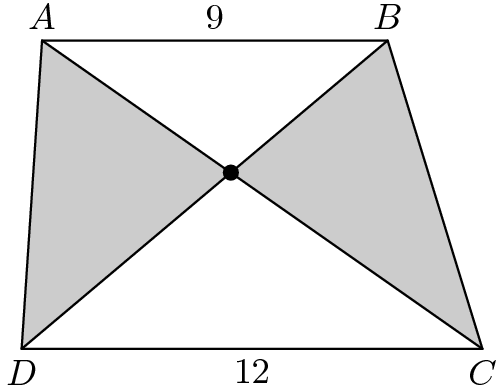
\includegraphics[height=5cm,page=1]{2021-07-31-figure-08}
\end{center}
\bigskip
Using the sine area formula on triangles $AED$ and $BEC$, as $\angle AED = \angle BEC$, we see that
\begin{align*}
\frac{AE}{EC} = \frac{BE}{ED}
\end{align*}
Since $\angle AEB = \angle DEC$, triangles $AEB$ and $DEC$ are similar. Their ratio is $\frac {AB}{CD} = \frac {3}{4}$. Since $AE + EC = 14$, we must have $EC = 8$, so $AE = 6\ \textbf{(E)}$. 
\begin{empheq}[box={\mathbox[colback=white]}]{equation*}
    6
\end{empheq} 
\end{answer}
%%%%%%%%%%%%%%%%%%%%%%%%%%%%%%%%%%%%%%%%%%%%%%%%%%%%%%%%%%%%%%%%%%%%%%%%

\iftoggle{showAnswers}{\newpage}

%%%%%%%%%%%%%%%%%%%%%%%%%%%%%%%%%%%%%%%%%%%%%%%%%%%%%%%%%%%%%%%%%%%%%%%%
\subsection*{8.}

\nopagebreak

Quadrilateral $ABCD$ has $AB = BC = CD$, $\angle ABC = 70^\circ$, and $\angle BCD = 170^\circ$. What is the degree measure of $\angle BAD$?

\fbox{(A) $75$ \quad (B) $80$ \quad (C) $85$ \quad (D) $90$ \quad (E) $95$}

\begin{answer}
This solution requires the use of cyclic quadrilateral properties but could be a bit time-consuming during the contest. To start off, draw a diagram like in solution one and label the points. Now draw $\overline{AC}$ and $\overline{BD}$ and call their intersection point $Y$. Note that triangle $BCD$ is an isosceles triangle so angles $CDB$ and $CBD$ are each $5$ degrees. Since $AB$ equals $BC$, angle $BAC$ equals $55$ degrees, thus making angle $AYB$ equal to $60$ degrees. We can also find out that angle $CYB$ equals $120$ degrees. Extend point $C$ such that it lies on the same level of segment $AB$. Call this point $E$. Since angle $BEC$ plus angle $CYB$ equals $180$ degrees, quadrilateral $YCEB$ is a cyclic quadrilateral. Next, draw a line from point $Y$ to point $E$. Since angle $YBC$ and angle $YEC$ point to the same arc, angle $YEC$ is equal to $5$ degrees. Since $EYD$ is an isosceles triangle (based on angle properties) and $YAE$ is also an isosceles triangle, we can find that $YAD$ is also an isosceles triangle. Thus, each of the other angles is $\frac{180-120}{2}=30$ degrees. Finally, we have angle $BAD$ equals $30+55=85$ degrees. 
\begin{empheq}[box={\mathbox[colback=white]}]{equation*}
    85 ~\text{degrees}
\end{empheq} 
\end{answer}
%%%%%%%%%%%%%%%%%%%%%%%%%%%%%%%%%%%%%%%%%%%%%%%%%%%%%%%%%%%%%%%%%%%%%%%%

\iftoggle{showAnswers}{\newpage}

%%%%%%%%%%%%%%%%%%%%%%%%%%%%%%%%%%%%%%%%%%%%%%%%%%%%%%%%%%%%%%%%%%%%%%%%
\subsection*{9.}

\nopagebreak

Two distinct regular tetrahedra have all their vertices among the vertices of the same unit cube. What is the volume of the region formed by the intersection of the tetrahedra?

\fbox{(A) $\dfrac{1}{12}$ \quad (B) $\dfrac{\sqrt{2}}{12}$ \quad (C) $\dfrac{\sqrt{3}}{12}$ \quad (D) $\dfrac{1}{6}$ \quad (E) $\dfrac{\sqrt{2}}{6}$}

\begin{answer}
\bigskip
\begin{center}
  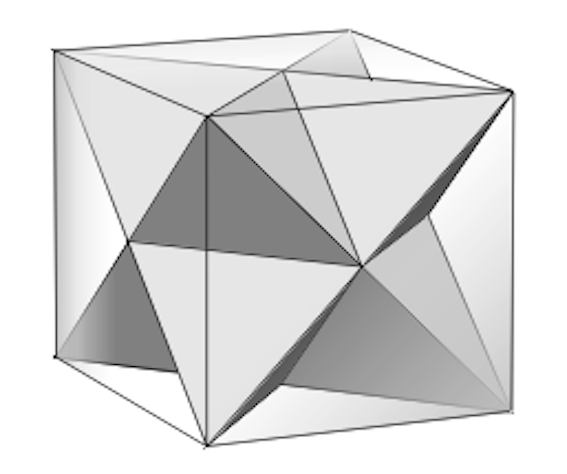
\includegraphics[height=5cm,page=1]{2021-07-31-figure-09}
\end{center}

A regular unit tetrahedron can be split into eight tetrahedra that have lengths of $\frac{1}{2}$. The volume of a regular tetrahedron can be found using base area and height:

For a tetrahedron of side length 1, its base area is $\frac{\sqrt{3}}{4}$, and its height can be found using Pythagoras' Theorem. Its height is
\begin{align*}
\sqrt{1^2-\left(\frac{\sqrt3}{3}\right)^2}=\frac{\sqrt2}{\sqrt3}
\end{align*}
Its volume is
\begin{align*}
\frac13\times\frac{\sqrt{3}}{4}\times\frac{\sqrt2}{\sqrt3}=\frac{\sqrt{2}}{12}
\end{align*}
The tetrahedron actually has side length $\sqrt2$, so the actual volume is
\begin{align*}
\frac{\sqrt{2}}{12}\times\sqrt2^3 = \frac{1}{3}
\end{align*}

On the eight small tetrahedra, the four tetrahedra on the corners of the large tetrahedra are not inside the other large tetrahedra. Thus, $\frac{4}{8}=\frac{1}{2}$ of the large tetrahedra will not be inside the other large tetrahedra.

The intersection of the two tetrahedra is thus
\begin{align*}
\frac{1}{2} \times \frac{1}{3} = \frac{1}{6}
\end{align*}
\begin{empheq}[box={\mathbox[colback=white]}]{equation*}
    \frac{1}{6}
\end{empheq} 
\end{answer}
%%%%%%%%%%%%%%%%%%%%%%%%%%%%%%%%%%%%%%%%%%%%%%%%%%%%%%%%%%%%%%%%%%%%%%%%

\iftoggle{showAnswers}{\newpage}

%%%%%%%%%%%%%%%%%%%%%%%%%%%%%%%%%%%%%%%%%%%%%%%%%%%%%%%%%%%%%%%%%%%%%%%%
\subsection*{10.}

\nopagebreak

In trapezoid $ABCD$ with bases $AB$ and $CD$, we have $AB = 52$, $BC = 12$, $CD = 39$, and $DA = 5$. The area of $ABCD$ is

\bigskip
\begin{center}
  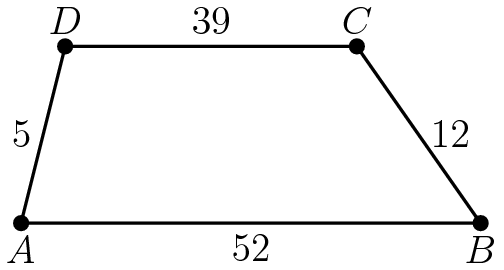
\includegraphics[width=5cm,page=1]{2021-07-31-figure-10}
\end{center}
\bigskip

\fbox{(A) $182$ \quad (B) $195$ \quad (C) $210$ \quad (D) $234$ \quad (E) $260$}

\begin{answer}
Extend $\overline{AD}$ and $\overline{BC}$ to meet at point $E$: 
\bigskip
\begin{center}
  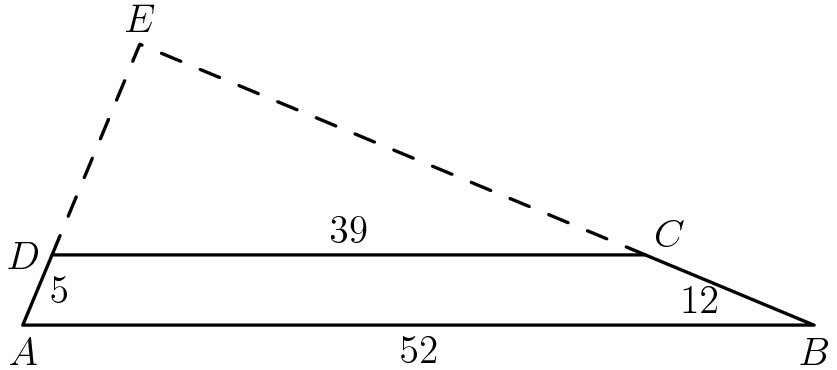
\includegraphics[width=8cm,page=1]{2021-07-31-figure-10b}
\end{center}
\bigskip
Since $\overline{AB} || \overline{CD}$ we have $\triangle AEB \sim \triangle DEC$, with the ratio of proportionality being $\frac {39}{52} = \frac {3}{4}$. Thus 
\begin{align*} 
\frac{CE}{CE+12} = \frac {3}{4} 
  & \Longrightarrow 
  CE = 36 \\ 
\frac{DE}{DE+5} = \frac {3}{4} 
  & \Longrightarrow 
  DE = 15 
\end{align*}
So the sides of $\triangle CDE$ are $15,36,39$, which we recognize to be a $5 - 12 - 13$ right triangle. Therefore (we could simplify some of the calculation using that the ratio of areas is equal to the ratio of the sides squared),
\begin{align*}
[ABCD] = [ABE] - [CDE] 
  = \frac {1}{2}\cdot 20 \cdot 48 - \frac {1}{2} \cdot 15 \cdot 36 
  = 210
\end{align*}
\begin{empheq}[box={\mathbox[colback=white]}]{equation*}
    210
\end{empheq} 
\end{answer}
%%%%%%%%%%%%%%%%%%%%%%%%%%%%%%%%%%%%%%%%%%%%%%%%%%%%%%%%%%%%%%%%%%%%%%%%

\iftoggle{showAnswers}{\newpage}

\end{document}
